\section{Subprogramas en Verilog: Funciones y tareas \label{sec:s3}}

\begin{center}
	\begin{minipage}{12cm}
		\begin{tcolorbox}[title=Actividad 1]
			Codificar en verilog la versión del circuito de los tres sumadores usando primero una función (function) y después usando una tarea (task).Compilar y simular.
		\end{tcolorbox}	
	\end{minipage}
\end{center}

La visualización RTL de los 3 sumadores de 4 bits en Verilog se muestra en la \autoref{fig:subprogram_3_adders_rtl}. Como se observa, la implementación se realiza utilizando 3 instancias de sumadores de 4 bits, independientes una de otra. Las simulaciones se visualizan en la \autoref{fig:subprogram_3_adders_wavebi} en base binaria y en la \autoref{fig:subprogram_3_adders_wavede} en base decimal, en donde se muestra que la suma se hace de manera correcta en cada elemento.

En los Anexos se localiza la descripción de los 3 sumadores de 4 bits. Las 2 implementaciones solo comparten la misma declaración de entradas y salidas del módulo.

\begin{itemize}
	\item \textbf{Para el caso de la función:} Se usa la palabra reservada \textit{function} y se declara en esa misma linea el tipo de valor que va a retornar, así como el nombre de la función. Después se declaran a las entradas y en el cuerpo se describe la operación de suma. Finalmente, dentro de una lista sensible se llama a la función, asignando el valor de retorno a la señal de salida correspondiente.
	\item \textbf{Para el caso de la tarea:} Se usa la palabra reservada \textit{task} y se coloca el nombre de la tarea. Después se declaran a las entradas y salidas y en el cuerpo se describe la operación de suma. Finalmente, dentro de una lista sensible se llama a la tarea, unicamente colocando a las señales como parámetros de la tarea.
\end{itemize}

\begin{figure}[ht]
	\centering
	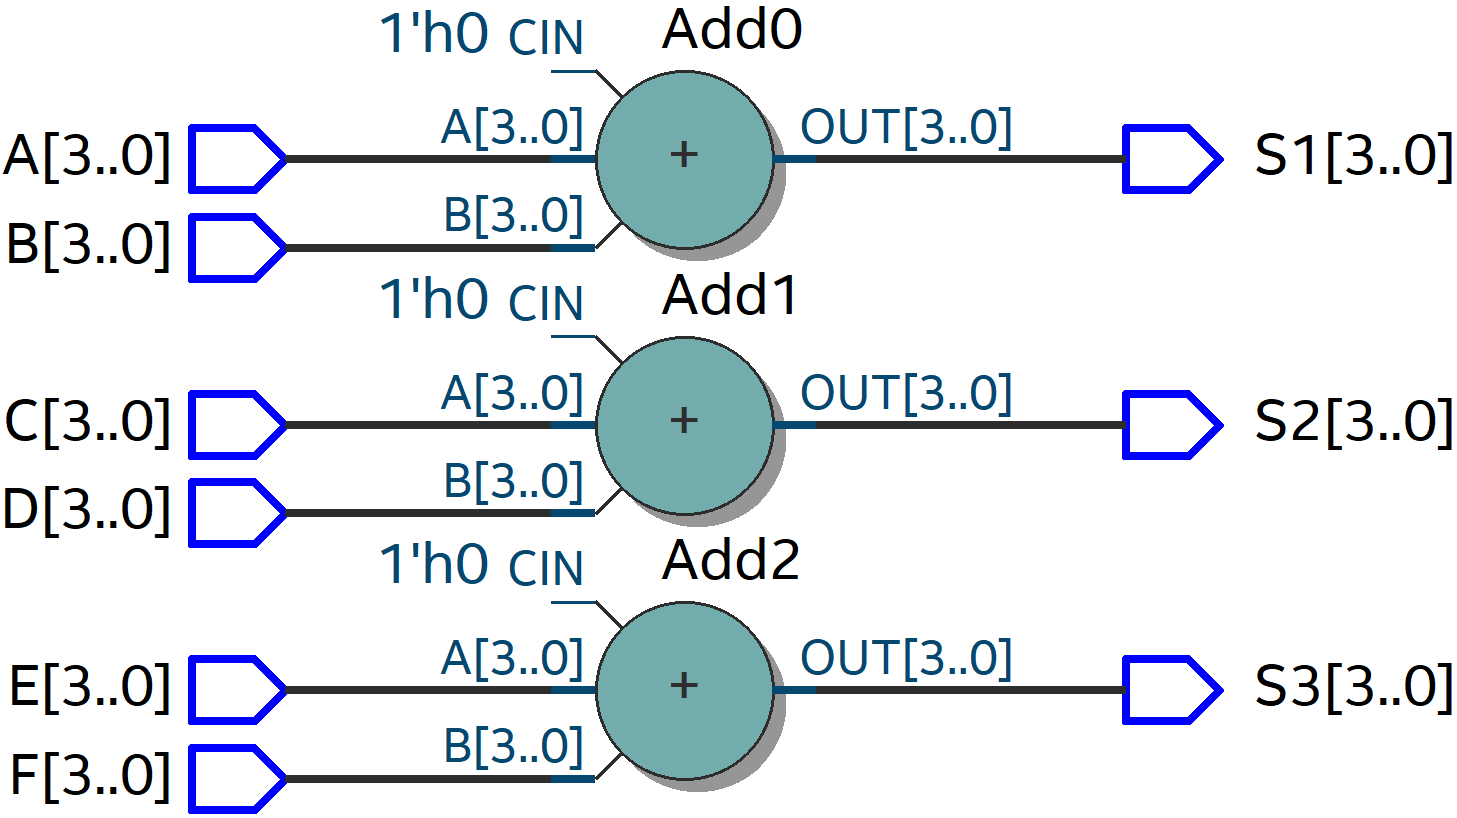
\includegraphics[scale=0.3]{Subprogram_3_Adders_RTL.png}
	\caption{Diagrama RTL de los 3 sumadores de 4 bits implementados en Verilog. Se tiene el mismo resultado si se usan funciones o tareas. \label{fig:subprogram_3_adders_rtl}}
\end{figure}

\begin{figure}[ht]
	\centering
	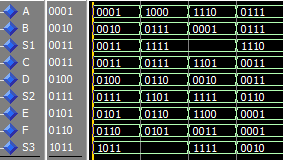
\includegraphics[scale=1]{Subprogram_3_Adders_WaveBi.png}
	\caption{Simulación de los 3 sumadores de 4 bits con el visor de formas de onda de ModelSim (base binaria). \label{fig:subprogram_3_adders_wavebi}}
\end{figure}

\begin{figure}[ht]
	\centering
	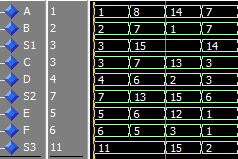
\includegraphics[scale=1]{Subprogram_3_Adders_WaveDe.png}
	\caption{Simulación de los 3 sumadores de 4 bits con el visor de formas de onda de ModelSim (base decimal). \label{fig:subprogram_3_adders_wavede}}
\end{figure}